\section{Conversion and the Appearance of the Input}
\label{app:details}
\label{app:appearance}

What changes before a model sees the scene? Conversion replaces material
networks while retaining meshes, object transforms, and scene composition.
ConvertAsset follows USD references, payloads, sublayers, and variants and
writes converted sibling layers; references in those layers point to their
converted counterparts. The source scenes remain available as the original
condition. Base color, roughness, metallic response, normal maps, and texture
connections are mapped into UsdPreviewSurface. Richer material effects are
examined separately in Appendix~\ref{app:materials}.

\subsection{Matched object views}
The object comparison contains four chest-of-drawers assets, each rendered from
six directions: front, back, left, right, and two elevated front views.
Table~\ref{tab:app-proxy} reports all 24 pairs. PSNR measures pixel error;
SSIM measures local luminance and contrast structure \citep{Wang2004Image};
LPIPS uses learned perceptual features \citep{Zhang2018Unreasonable}.
CLIP and DINOv2 cosine similarities compare image embeddings
\citep{Radford2021Learning,Oquab2023DINOv2}.

\begin{table}[htbp]
\centering\small
% Generated by appendix/build_tables.py; source hashes in table_sources.json.
\begin{tabular}{lrrrrrr}
\toprule
Asset & Pairs & PSNR & SSIM & LPIPS & CLIP & DINOv2 \\
\midrule
Chest 0004 & 6 & 37.51 & 0.991 & 0.019 & 0.921 & 0.798 \\
Chest 0011 & 6 & 36.30 & 0.993 & 0.017 & 0.956 & 0.922 \\
Chest 0023 & 6 & 30.59 & 0.986 & 0.032 & 0.938 & 0.905 \\
Chest 0029 & 6 & 37.68 & 0.991 & 0.014 & 0.885 & 0.864 \\
All & 24 & 35.52 & 0.990 & 0.020 & 0.925 & 0.872 \\
\bottomrule
\end{tabular}

\caption{Matched object renders, averaged over six views per asset. PSNR is
in dB; higher PSNR, SSIM, CLIP, and DINOv2 indicate greater similarity, while
lower LPIPS indicates greater similarity.}
\label{tab:app-proxy}
\end{table}

The averages are high, but the per-asset results preserve useful differences.
Chest 0023 has the lowest PSNR and highest LPIPS, whereas Chest 0004 has the
lowest DINOv2 similarity. Pixel agreement and feature agreement thus emphasize
different aspects of the same paired images. Figures~\ref{fig:app-proxy1}
and~\ref{fig:app-proxy2} retain object context across camera directions so these
measurements can be read alongside the visible surfaces.

For images scaled to $[0,1]$, PSNR is $10\log_{10}(1/\mathrm{MSE})$.
The LPIPS implementation uses a VGG backbone. Feature measurements use
CLIP ViT-B/32 and DINOv2 image embeddings, with cosine similarity
$f(I^O)^\top f(I^C)/(\|f(I^O)\|_2\|f(I^C)\|_2)$.
Each reported mean weights the recorded views equally.

\subsection{From objects to scene context}
Figure~\ref{fig:app-scene} shows paired GRScenes views. Materials affect several
parts of an observation at once: the target surface, the nearby background,
and reflected illumination. These views motivate the full-image and window
comparisons in the main paper. The object metrics describe the four-asset
render set; the scene views show the visual inputs from which the grounding
experiments were developed.

\begin{figure}[p]
\centering
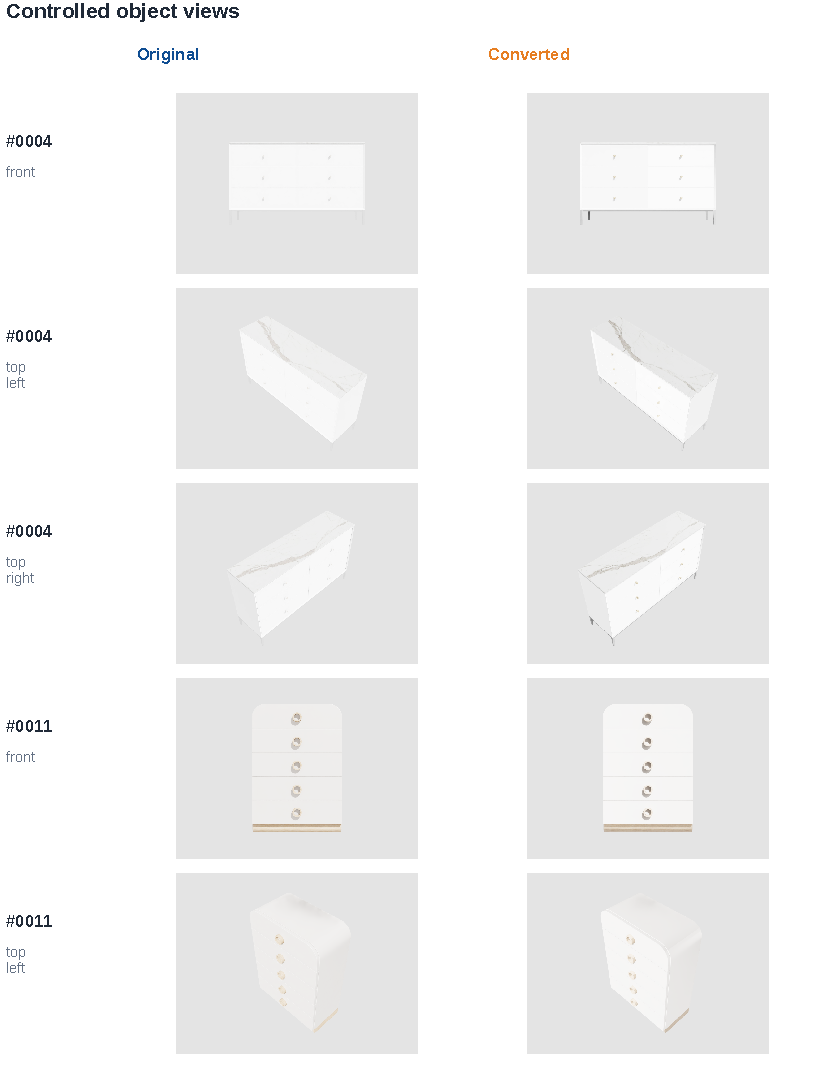
\includegraphics[width=\linewidth,height=.84\textheight,keepaspectratio]{appendix_render_pairs_01.pdf}
\caption{Original and converted object views from the four-asset render set. Each pair shows the same camera direction, retaining full object context.}
\label{fig:app-proxy1}
\end{figure}

\begin{figure}[p]
\centering
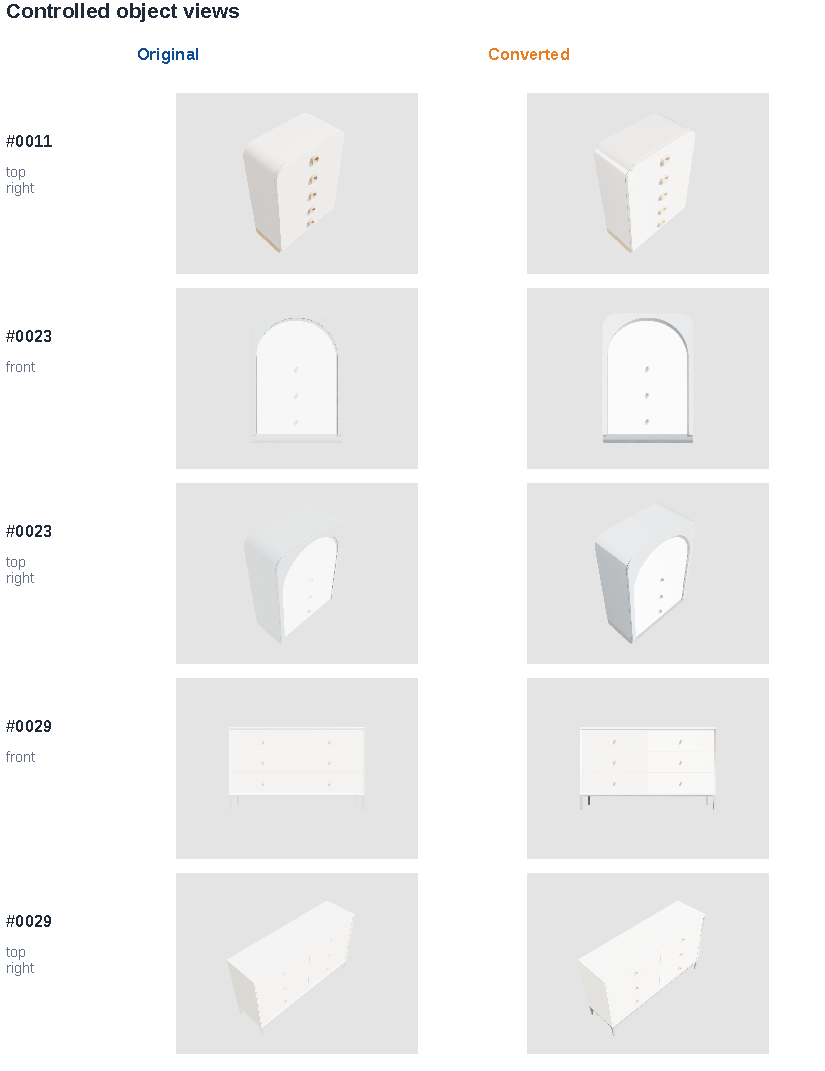
\includegraphics[width=\linewidth,height=.84\textheight,keepaspectratio]{appendix_render_pairs_02.pdf}
\caption{Additional camera directions for the four-asset paired render set. The six-view measurements for every asset appear in Table~\ref{tab:app-proxy}.}
\label{fig:app-proxy2}
\end{figure}

\begin{figure}[p]
\centering
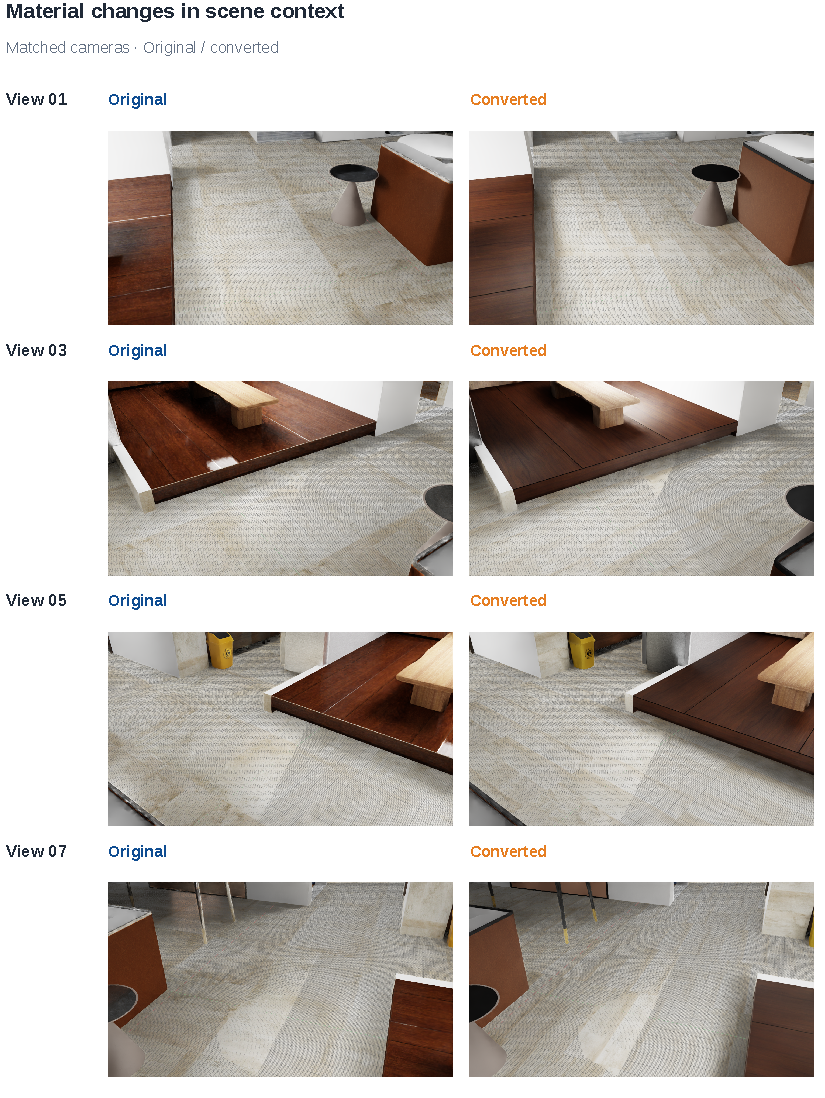
\includegraphics[width=\linewidth,height=.84\textheight,keepaspectratio]{appendix_scene_pairs.pdf}
\caption{Paired GRScenes camera views under original and converted materials. Scene layout is shared while surface appearance and illumination cues change.}
\label{fig:app-scene}
\end{figure}
\FloatBarrier
